\documentclass[titlepage]{article}
\usepackage{graphicx}
\usepackage{listings}
\usepackage{color}
\usepackage{gensymb}

\definecolor{dkgreen}{rgb}{0,0.6,0}
\definecolor{gray}{rgb}{0.5,0.5,0.5}
\definecolor{mauve}{rgb}{0.58,0,0.82}
\makeatletter
\setlength{\@fptop}{0pt}
\makeatother

\lstset{frame=tb,
  language=Java,
  aboveskip=3mm,
  belowskip=3mm,
  showstringspaces=false,
  columns=flexible,
  basicstyle={\small\ttfamily},
  numbers=none,
  numberstyle=\tiny\color{gray},
  keywordstyle=\color{blue},
  commentstyle=\color{dkgreen},
  stringstyle=\color{mauve},
  breaklines=true,
  breakatwhitespace=true,
  tabsize=3
}

\title{CS440 - Artificial Intelligence \\ Assignment 1 (3 Credit Hours)}
\author{Jon Reynolds (jdrynld2) \\ Matthew Krikorian (krikorn2) \\ Patrick McMahon (pfmcmah2)}

\begin{document}

\maketitle

\section{Abstract}
In this assignment we explore the different search algorithms that can be used to traverse a maze, and analyze the optimality's and general performance between the different implementations under a very heavy scope. In section 1.1 (basic pathfinding), we analyzed four different pathfinding algorithms. Specifically, Depth-first search, Breadth-first search, Greedy best-first search, and A* search. In section 1.2 (search with multiple dots), we were tasked with developing our own heuristic in the implementation of our A* search algorithm. There are also multiple goal positions in section 1.2 as well, which is why coming up with an admissible heuristic to optimally traverse the mazes was paramount.

\section{Section 1.1, Basic Pathfinding} 

\subsection{Search Algorithms, Explained}
In this part of the assignment we implemented four different search algorithms to analyze cost, number of nodes expanded, and overall solution optimality. We were given three different mazes to run our search algorithms on, demonstrating to us the potential pros and cons of each algorithm. \textbf{Breadth-first search} is a search algorithm where the root node is expanded first, then all of the root-notes children are expanded, and so forth until the goal successor (or state) is found. 

\begin{figure}[h!]
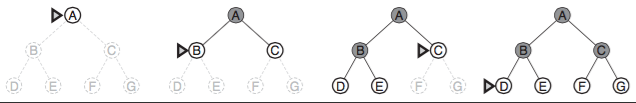
\includegraphics[width=\linewidth]{bfs.png}
\caption{Breadth-first search algorithm, \textit{Russell and Norvig}}
\label{fig:BFSdiagram1}
\end{figure}

\noindent
\textbf{Depth-first search} is a search algorithm where the deepest node currently in the frontier is always chosen to be expanded with the hope of finding the goal state. If the goal state is not found once the algorithm finds a node with no successors, the algorithm will then backtrack back to the next deepest node that still has unexplored successors.

\newpage

\begin{figure}[h!]
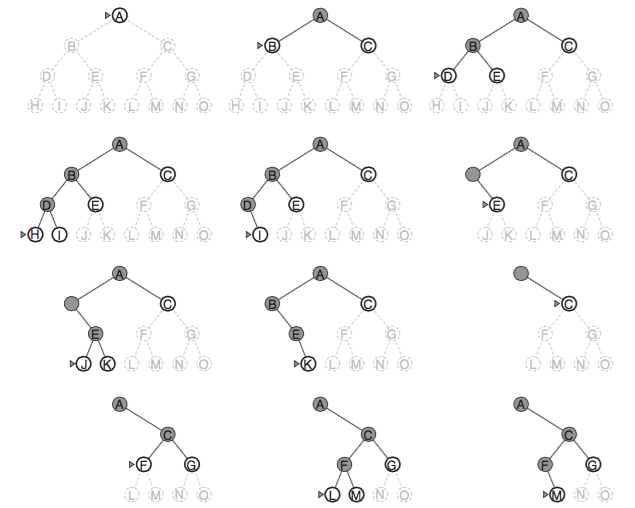
\includegraphics[width=\linewidth]{dfs.png}
\caption{Depth-first search algorithm, \textit{Russell and Norvig}}
\label{fig:DFSdiagram1}
\end{figure}

\noindent
\textbf{Greedy best-first search} is a search algorithm that always chooses to go down the path that has the lowest cost with respect to the other neighbors of the current node it is on. The name greedy implies that it does not care about the actions of the future, but rather only chooses it's path on the best choice to it based on immediate cost. Greedy algorithms evaluate the nodes they are going to travel to using a heuristic function. This heuristic does not use past or future information to make any decisions, which sets it apart from both the BFS and DFS search algorithms. The algorithm chooses the next node it will travel to directly from the heuristic function it is given, so the choosing function \(f(n)\) can be modeled as \(f(n) = h(n)\) where \(h(n)\) is the heuristic function.\newline
\newline
Finally, \textbf{A* search} is a search algorithm where the function used to evaluate which node the algorithm will travel to next, \(f(n)\), is dependent on both the cost from the start node to the current node, \(g(n)\), and the cost to get from the current node to the goal node, \(h(n)\). The node selection function is actually modeled as the direct sum of \(h(n)\) and \(g(n)\), giving us \(f(n) = h(n) + g(n)\). This algorithm is thought of as the algorithm amongst the four that often provides the most savings, and can be optimized heavily through a very good heuristic function \(h(n)\).

\subsection{Our Code, Explained}
Our assignment is broken up into a \textit{src} folder which holds all of our \textit{.cpp} files, our \textit{include} folder holds all of the \textit{.h} files that we wrote, our \textit{build} folder holds all of the \textit{.o} files that are used in compilation, our \textit{bin} folder contains all of the \textit{.exe} files that we use to execute our search algorithms, and the \textit{tex} folder holds all of the \textit{.tex} that was used to compile the pdf that we submitted. 
\subsubsection{\textit{frontier.cpp} and \textit{frontier.h}}
The file which handles keeping track of the frontier is \textit{frontier.cpp} and \textit{frontier.h}. Here we define a FrontierNode that acts as a wrapper for nodes that are kept in the running solution of the maze. The struct is defined as below.

\begin{lstlisting}
struct FrontierNode{
    Node* node;
    Node* prevNode;
    FrontierNode* next;
    FrontierNode* prev;
    int pathCost;
    int heuristic;
};
\end{lstlisting}

During traversal, FrontierNodes are kept in a doubly linked-list so that adding and removing nodes that are deemed to not be a part of the solution can be removed easily. For example, when we perform Depth-first search, FrontierNodes are added to the linked list until the algorithm realizes there is no deeper node to traverse to, in which case we back-track and remove the last FrontierNode from the linked list and backtrack back to a FrontierNode where \textit{prev} points to a FrontierNode that wraps a Node that has an unexplored Node. The FrontierNode struct also keeps track of the pathCost for the given node, as well as a value for that FrontierNode based on the heuristic function being used. In \textit{frontier.cpp} and \textit{frontier.h}, we define a Frontier class that holds all of the functions used to modify the frontier while traversing the maze. 

\begin{lstlisting}
class Frontier {
public:
    Frontier();
    ~Frontier();
    void push_back(Node* node, Node* prevNode, int val=0, int cost = 0);
    void push_front(Node* node, Node* prevNode, int val=0, int cost=0);
    FrontierNode* pop_back(std::unordered_map<Node*, Node*>& history);
    FrontierNode* pop_front(std::unordered_map<Node*, Node*>& history);
    FrontierNode* pop_min(std::unordered_map<Node*, Node*>& history);
    FrontierNode* getHead();
    FrontierNode* getTail();
    bool empty();
    FrontierNode* find(Node* node);
    void update(FrontierNode* fnode);

private:
    FrontierNode* head;
    FrontierNode* tail;
    int size;
    std::unordered_map<Node*, FrontierNode*> nodeMap;
\end{lstlisting}

The various push and pop functions in our Frontier class are used to easily manage the stack and queue when implementing DFS and BFS. When implementing DFS, we used a stack data structure to easily remove the most recently added nodes from the top of the stack. For Greedy and A* search, \textit{pop min} is used to find the lowest cost option for finding the next node based on each algorithms node choosing function. 

\subsubsection{\textit{maze.cpp} and \textit{maze.h}}
\begin{lstlisting}
class Maze {

public:
    Maze(std::string filename, std::string version);
    ~Maze();
    Node* getStart();
    std::vector<Node*> getGoals();
    int getNumGoals();
    void printSolution();
    std::string getName();
    std::string getVersion();
    std::vector<Node*> getNeighbors(Node* cur, int numDots, uint32_t hash);
    void visit(Node* curNode);
    void setSymbol(Node* curNode, int place);
    bool canSetSymbol(Node* curNode);

private:
    std::string name, version;
    Node* start;
    std::vector<Node*> goals;
    std::unordered_map<uint32_t, Node*>**** maze;
    int w, h, numGoals;

};
\end{lstlisting}

The purpose of \textit{maze.cpp} and \textit{maze.h} in our assigment is to take in an inputted maze text file, parse it, and allocate a 2-dimensional matrix which holds all the information related to the contents of the maze. After extracting the contents of the maze and putting it in a 2-dimensional array, the maze class writes the data in the array into Nodes which store the essential information of each position of the maze. This class can be thought of as the maze creation class, initializing all of the Nodes that are going to be used in the \textit{main.cpp} file to build the frontier. This class also holds functions used to write to the maze in Section 1.2, such as setSymbol and canSetSymbol, which are used to label symbols on the multiple goal states in the later mazes we need to traverse.

\subsubsection{\textit{node.cpp} and \textit{node.h}}
\begin{lstlisting}
class Node {

public:
    Node(int x, int y, int numDots, uint32_t dotsHash, int dotId = -1);
    bool isVisited();
    void visit();
    bool isGoal();
    int getX();
    int getY();
    int getDots();
    uint32_t getDotsTakenHash();
    int getDotId();
    void setTaken(int dotNumber);
    bool hasTaken(int dotNumber);
    void setSymbol(int place);
    char getSymbol();
    bool canSet();

private:
    int x, y, numDots, dotId;
    uint32_t dotsHash;
    char symbol;
    bool visited, notSet;
    static const unsigned char* symbols;

};
\end{lstlisting}
The Node class is the basis of how the maze is traversed and information relevant to the maze is stored. Every node is initialized with an x and y coordinate value, the neighbors of the given node in the maze stored in a vector of Node pointers, and a boolean value that determines whether any given search algorithm has already visited that Node. The Node class along with the FrontierNode class are the foundational Nodes used to traverse the maze and store the solution that is to be printed after the algorithm is done searching for the goal state. The third dimension of the array that keeps all the data in a node is populated with the numDots variable, which keeps track of how many dots have been collected in the traversal from that node. The symbols char is used to hold the character that is to be written at the designated maze location for Section 1.2, as well as the setSymbol and getSymbol functions.

\subsubsection{\textit{main.cpp}}
This file is the body where all of the Nodes and FrontierNodes are processed and the main algorithms are implemented. This file is where the functions to manage the stack for Depth-first search is managed as well as the queue for Breadth-first search are called and the overall algorithm for those two algorithms is implemented. This file is also where the solution frontier for both Greedy and A* Search are maintained and handled, and the manhattan distance heuristic is used to properly calculate the next Node to be traversed. We've also implemented the backtracking in this file which handles re-visiting the last Node with unexplored neighbors. After each maze is traversed and a solution is found, this file then goes and prints the respective solutions for each maze.

\newpage

%% DFS subsection 
\subsection{Depth-First Search Outputs}
Below are the outputs we generated for each maze using the Depth-first search algorithm. 
\subsubsection{Medium Maze}
\begin{figure}[h!]
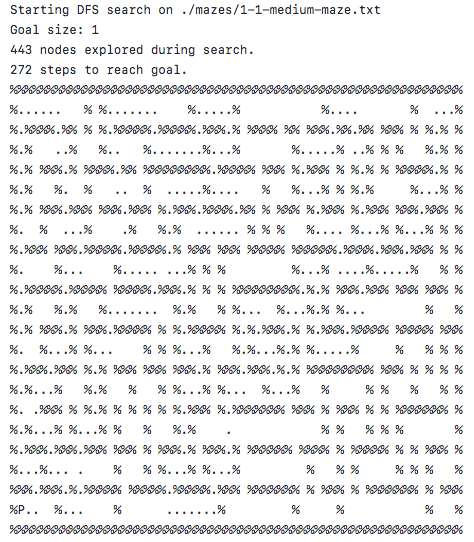
\includegraphics[width=\linewidth]{dfsmedium.png}
\caption{Depth-first search on the medium maze}
\label{fig:DFSmedium}
\end{figure}

\newpage
\subsubsection{Big Maze}
\begin{figure}[h!]
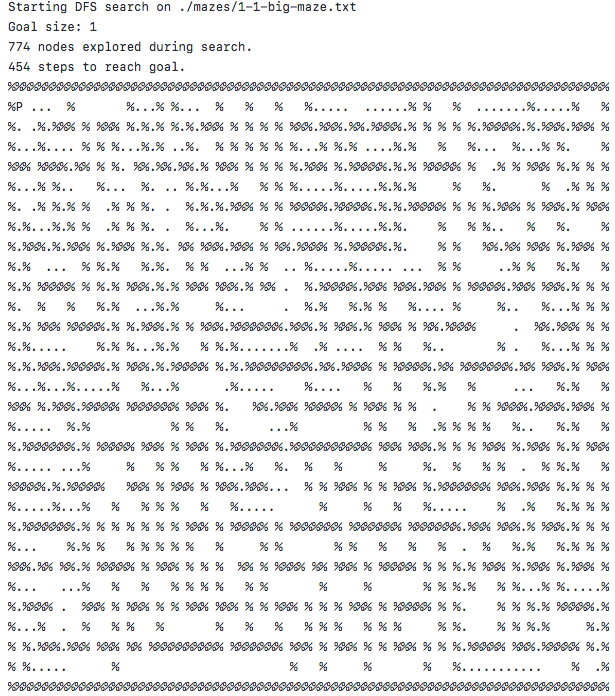
\includegraphics[width=\linewidth]{dfsbig.png}
\caption{Depth-first search on the big maze}
\label{fig:DFSbig}
\end{figure}

\newpage

\subsubsection{Open Maze}
\begin{figure}[h!]
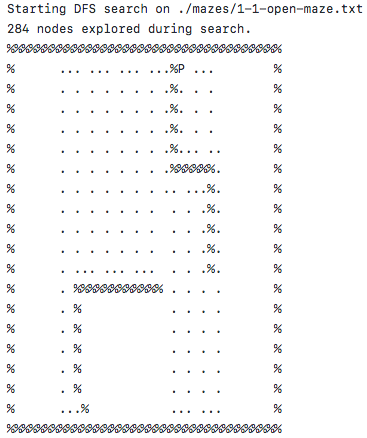
\includegraphics[width=\linewidth]{dfsopen.png}
\caption{Depth-first search on the open maze}
\label{fig:DFSopen}
\end{figure}

\newpage
%%BFS Section
\subsection{Breadth-First Search Outputs}
Below are the outputs we generated for each maze using the Breadth-first search algorithm. 
\subsubsection{Medium Maze}
\begin{figure}[h!]
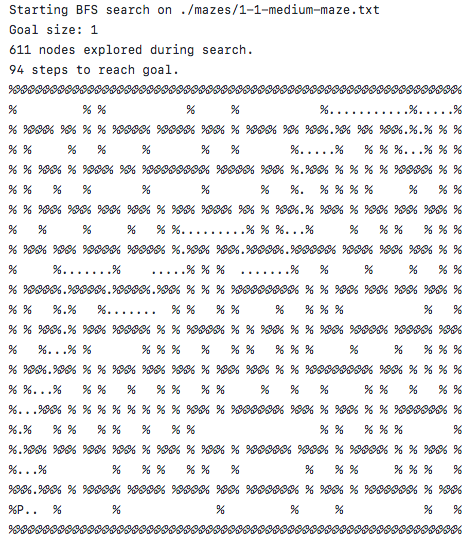
\includegraphics[width=\linewidth]{bfsmedium.png}
\caption{Breadth-first search on the medium maze}
\label{fig:BFSmedium}
\end{figure}

\newpage
\subsubsection{Big Maze}
\begin{figure}[h!]
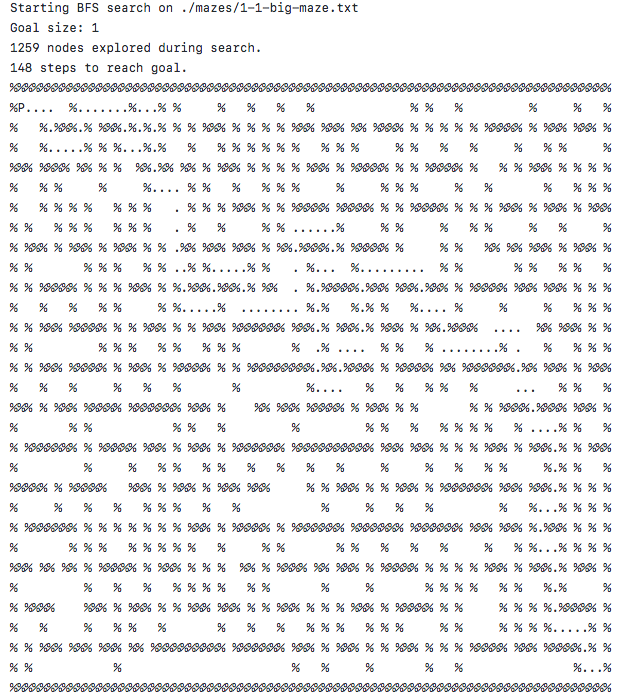
\includegraphics[width=\linewidth]{bfsbig.png}
\caption{Breadth-first search on the big maze}
\label{fig:BFSbig}
\end{figure}

\newpage

\subsubsection{Open Maze}
\begin{figure}[h!]
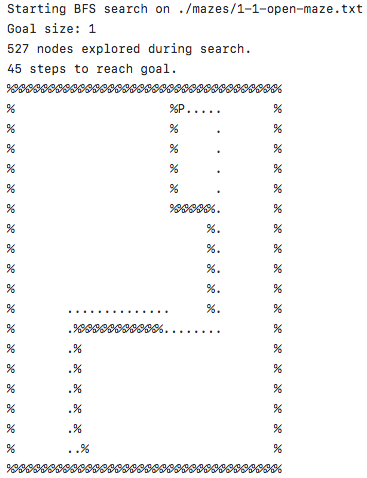
\includegraphics[width=\linewidth]{bfsopen.png}
\caption{Breadth-first search on the open maze}
\label{fig:BFSopen}
\end{figure}

\newpage

%%Greedy boys
\subsection{Greedy Search Outputs}
Below are the outputs we generated for each maze using the Greedy search algorithm. 
\subsubsection{Medium Maze}
\begin{figure}[h!]
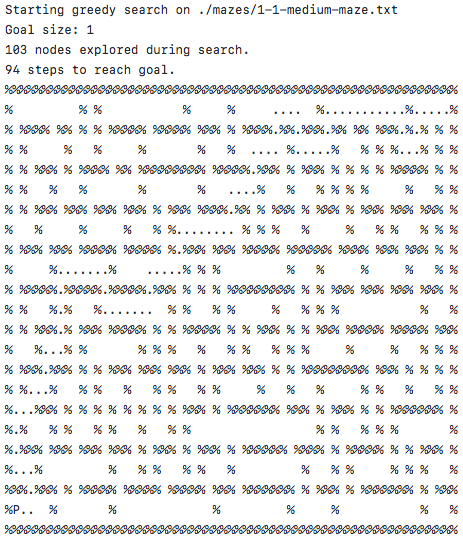
\includegraphics[width=\linewidth]{greedymedium.png}
\caption{Greedy search on the medium maze}
\label{fig:GREEDYmedium}
\end{figure}

\newpage
\subsubsection{Big Maze}
\begin{figure}[h!]
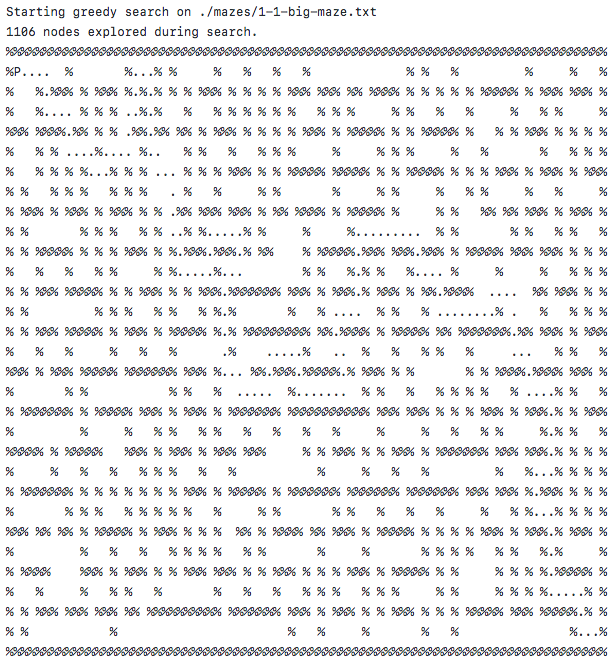
\includegraphics[width=\linewidth]{greedybig.png}
\caption{Greedy search on the big maze}
\label{fig:GREEDYbig}
\end{figure}

\newpage

\subsubsection{Open Maze}
\begin{figure}[h!]
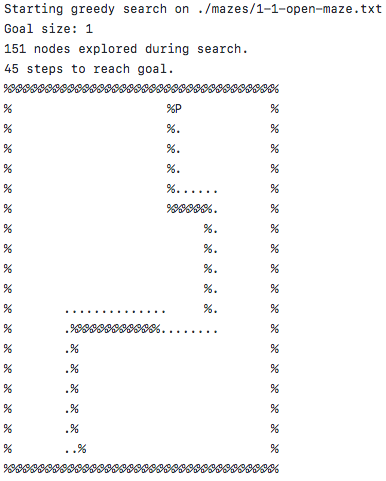
\includegraphics[width=\linewidth]{greedyopen.png}
\caption{Greedy search on the open maze}
\label{fig:GREEDYopen}
\end{figure}

\newpage

%%A* boys
\subsection{A* Search Outputs}
Below are the outputs we generated for each maze using the A* search algorithm. 
\subsubsection{Medium Maze}
\begin{figure}[h!]
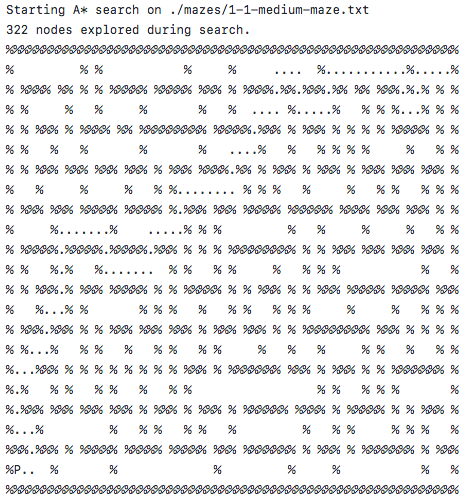
\includegraphics[width=\linewidth]{astarmedium.png}
\caption{A* search on the medium maze}
\label{fig:ASTARmedium}
\end{figure}

\newpage
\subsubsection{Big Maze}
\begin{figure}[h!]
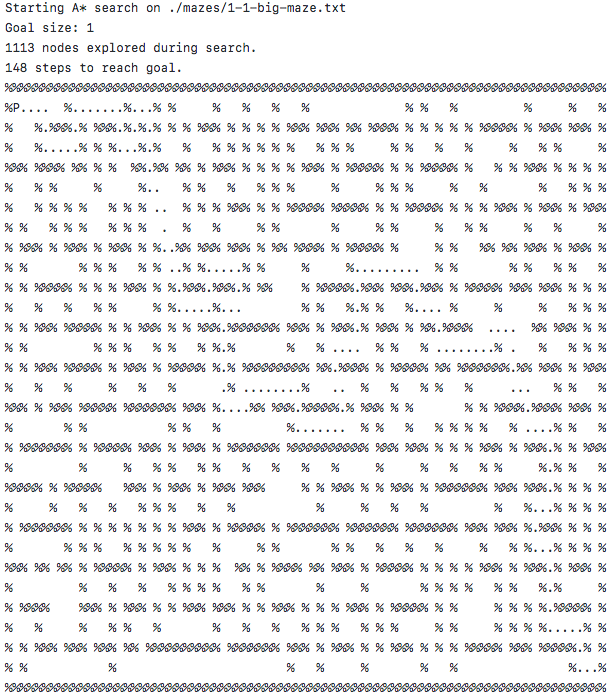
\includegraphics[width=\linewidth]{astarbig.png}
\caption{A* search on the big maze}
\label{fig:ASTARbig}
\end{figure}

\newpage

\subsubsection{Open Maze}
\begin{figure}[h!]
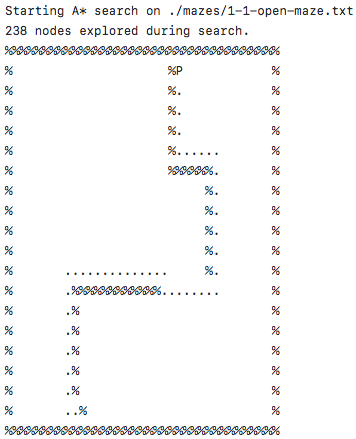
\includegraphics[width=\linewidth]{astaropen.png}
\caption{A* search on the open maze}
\label{fig:ASTARopen}
\end{figure}

\newpage

\subsection{Manhattan Distance Heuristic, Explained}
The Manhattan Distance is what we used to calculate the heuristic function. This function was then compared to the actual value of the heuristic function at that node, and used to make sure the FrontierNode stored in the minHeap is correct. The Manhattan Distance formula is as follows:

\[ |Node_{x, 1} - Node_{x, 2}| + |Node_{y, 1} - Node_{y, 2}|   \]

\noindent
This heuristic is used when an algorithm must traverse a setting in which it can only make 90\degree turns, which makes sense given the name is derived from the way one would traverse New York City if walking on foot. The streets and avenues are all perpendicular to one another, so one traversing the city would use the same heuristic as both the Greedy and A* search algorithms did in our assignment. Every node pushed onto the frontier has the Manhattan Distance of its neighbors calculated, and the node with the best path-cost to the goal state is pushed onto the frontier. We also use the Manhattan Distance in both the Greedy and A* search algorithms to determine if the Node at the top of the minHeap has the lowest cost to the goal state, because Manhattan Distance is the heuristic used for both of those search algorithms. Greedy depends entirely on the Manhattan Distance heuristic, while A* sums it with the path cost of the starting node to the current node.

\subsection{Summary and Closing Points}
As said before, we used a stack to manage the nodes the that will be part of the solution for our Depth-first search algorithm, we used a queue to manage the nodes used in our Breadth-first search algorithm, and then a Priority Queue that we wrote from scratch to manage the solution path for both Greedy search and A* search. We also used a minNodeHeap to keep track of the frontier nodes that acted as wrappers for nodes that were to be included in the solution. The top node of the minNodeHeap was always the node with the suspected lowest path cost calculated differently based on which algorithm was being used. For Greedy search, it strictly used the Manhattan heuristic, for A* search is would take the sum of the heuristic and distance of the starting node to the current node. We'd remove the frontier node wrapping a certain node from the heap if the information related to the node changed and no longer made it part of the frontier, such as having an incorrect path cost. 

\newpage

\section{Section 1.2, Search With Multiple Dots} 
In Section 1.2, the plot thickens yet again. We are now told to evaluate mazes that are much smaller than the mazes in Section 1.1, however the mazes now have multiple goal states. The starting state of the mazes in this section start with 'P' and end have goal denoted by the '.' symbol. The difference this time is we can't draw the dots to represent the path our algorithm takes as it would be too costly, so what we do instead in our implementation in this section is to draw letters at each of the goal states in the order that the implementation arrives to that state. The goal states are represented with alpha-numerical characters for numbers \textit{1-9}, and then we begin to use the alphabetical characters \textit{a-z} once the \textit{9th} goal state is labeled. For debugging purposes we ran Breadth-first search on the tiny maze and the small maze, and then only ran our custom heuristic for A* on the medium maze. 

\subsection{Our Code, Explained}
\end{document}




























